\section{Sistema RAG e o acervo de discursos parlamentares}\label{sec:caso}

Esta seção documenta o sistema RAG e o corpus de discursos da 56\textordfeminine{} Legislatura do Senado Federal empregados como caso empírico. O corpus já possui versão congelada e análise exploratória documentada. O protótipo técnico já implementado constitui o ponto de partida da análise de viabilidade; a configuração do sistema usada no experimento principal ainda deverá ser congelada e descrita de modo reproduzível, incluindo código, modelos, parâmetros e configurações.

\subsection{Caracterização do corpus legislativo}\label{sec:caracterizacao-corpus}

O corpus analisado reúne os pronunciamentos da 56\textordfeminine{} Legislatura abrangidos pela coleta descrita na seção metodológica. A fonte, a janela consultada, a versão do arquivo e os procedimentos de coleta e auditoria estão documentados na Seção de coleta e análise exploratória do corpus. Esta subseção apresenta os resultados descritivos da auditoria e discute suas implicações para a preparação e a avaliação do sistema RAG.

Dos 15.729 registros, 15.039 possuem texto integral, 687 dependem de resumo como fonte substituta e três não contêm texto nem resumo utilizável. Assim, 15.726 registros, ou 99,98\%, têm algum conteúdo indexável, mas texto integral e resumo não serão tratados como evidências equivalentes. A proveniência deverá acompanhar cada unidade recuperável para permitir que a avaliação distinga a fonte documental utilizada. Também foram identificadas 28 cópias textuais exatas excedentes, 1.291 documentos com menos de 50 palavras, sete documentos com mais de 10 mil palavras e cobertura de 86,81\% para partido e unidade federativa entre os documentos indexáveis. Esses achados recomendam inspeção antes de deduplicação, tratamento explícito de documentos curtos e longos e cautela no uso de filtros por metadados incompletos.

A estimativa de segmentação não criou unidades de recuperação reais. Com aproximação de 512 tokens por trecho e sobreposição de 64 tokens, a simulação estimou 45.971 trechos, mediana de dois trechos para textos integrais e máximo aproximado de 60. Configurações de 256, 768 e 1.024 tokens também foram simuladas para dimensionar o índice. Esses valores servem ao planejamento; a segmentação efetiva deverá usar o tokenizador do modelo escolhido, respeitar limites semânticos e ser comparada empiricamente no protocolo de recuperação.

A Tabela~\ref{tab:cobertura-corpus} apresenta a disponibilidade textual, distinguindo documentos integrais de resumos usados como substitutos. Essa distinção deve acompanhar a avaliação: uma resposta apoiada apenas em resumo não possui necessariamente a mesma cobertura documental de uma resposta apoiada no pronunciamento integral.

\begin{table}[htbp]
\centering
\caption{Disponibilidade textual dos registros do corpus.}\label{tab:cobertura-corpus}
\begin{tabular}{lrr}\toprule
Fonte disponível & Registros & Percentual (\%)\\\midrule
Texto integral & 15.039 & 95,61\\
Resumo substituto & 687 & 4,37\\
Sem conteúdo utilizável & 3 & 0,02\\\midrule
Total & 15.729 & 100,00\\\bottomrule
\end{tabular}
\par\smallskip Fonte: elaborado pelo autor a partir da análise exploratória do corpus, versão 1.1.1 (2026).
\end{table}

A Figura~\ref{fig:estimativa-segmentacao} compara estimativas do número de trechos sob quatro tamanhos e respectivas sobreposições. Reduzir o tamanho eleva o número estimado de unidades a indexar. A figura dimensiona o planejamento computacional; não demonstra melhoria de recuperação nem representa uma segmentação final executada.
\begin{figure}[htbp]
\centering
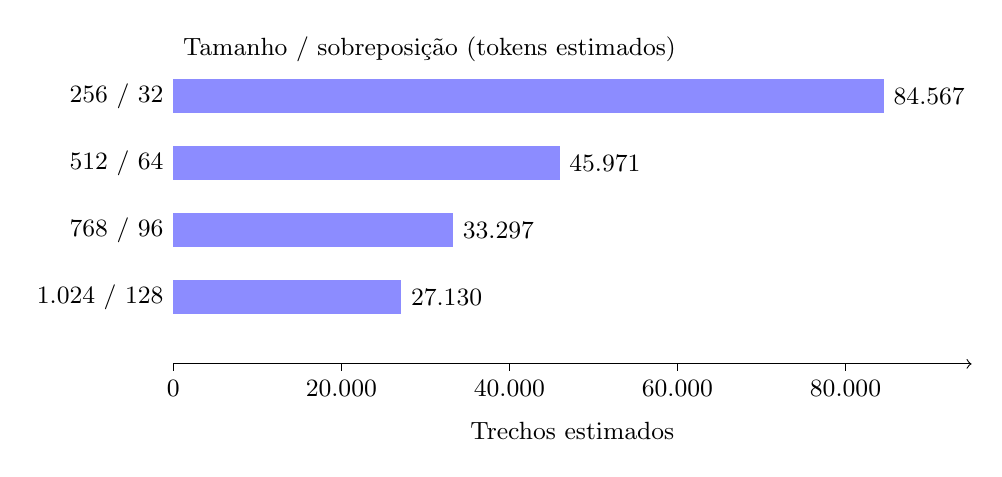
\begin{tikzpicture}[x=0.00011cm,y=0.85cm]
\draw[->] (0,0)--(95000,0);
\node[font=\small] at (47500,-1.0){Trechos estimados};
\foreach \v/\t in {0/0,20000/20.000,40000/40.000,60000/60.000,80000/80.000}{\draw (\v,0)--(\v,-0.1) node[below,font=\small]{\t};}
\foreach \y/\v/\t/\n in {4/84567/{256 / 32}/{84.567},3/45971/{512 / 64}/{45.971},2/33297/{768 / 96}/{33.297},1/27130/{1.024 / 128}/{27.130}}{
\fill[blue!45] (0,\y-0.25) rectangle (\v,\y+0.25);
\node[left,font=\small] at (0,\y){\t};
\node[right,font=\small] at (\v,\y){\n};}
\node[anchor=west,font=\small] at (0,4.7){Tamanho / sobreposição (tokens estimados)};
\end{tikzpicture}
\caption{Estimativa de segmentação do corpus por tamanho e sobreposição.}\label{fig:estimativa-segmentacao}
\par\smallskip Fonte: elaborado pelo autor a partir das saídas da análise exploratória (2026).
\end{figure}

A inspeção exploratória usou referências de planejamento: ao menos 99\% de registros com conteúdo utilizável, 90\% com texto integral, menos de 1\% sem conteúdo, menos de 2\% de cópias exatas excedentes e menos de 10\% com menos de 50 palavras. Os valores observados foram, respectivamente, 99,98\%, 95,61\%, 0,02\%, 0,18\% e 8,21\%. Esses limites foram empregados para identificar pontos de atenção, não para certificar qualidade do corpus ou do sistema. A cobertura de partido e unidade federativa, de 86,81\% entre documentos indexáveis, ficou abaixo da referência exploratória de 90\%; sua interpretação exige distinguir ausência de informação de não aplicabilidade desses campos a determinados autores. O resultado autoriza planejar experimentos controlados com ressalvas, sem antecipar desempenho de recuperação ou geração.

\subsection{Arquitetura e componentes do sistema RAG}

O protótipo de viabilidade combina scripts Python para preparação documental e avaliação, Open WebUI como interface e orquestrador do fluxo RAG e ChromaDB como armazenamento vetorial. A aplicação recebe a pergunta, recupera trechos da base indexada, encaminha o contexto ao modelo gerador e registra resposta, fontes e metadados para inspeção. Os artefatos de execução identificam a base de conhecimento pelo mesmo identificador nas quatro rodadas completas de 5 de maio de 2026; isso permite vincular os resultados registrados a uma configuração concreta do protótipo.

Essa arquitetura descreve a implementação examinada na viabilidade. O experimento principal deverá congelar separadamente o recuperador, o modelo de embeddings, o modelo gerador e os parâmetros de consulta, de modo que a comparação entre estratégias de recuperação mantenha constantes as demais condições relevantes.

\subsection{Preparação, segmentação e enriquecimento documental}

O manifesto de preparação da base de viabilidade registra 15.729 registros de entrada: 15.726 forneceram texto utilizável e três foram ignorados. O processo produziu 23.806 trechos, dos quais 23.119 derivam de textos integrais e 687 de resumos substitutos. A configuração foi limitada a 850 palavras por trecho, com sobreposição de 150 palavras e máximo de 200 trechos por arquivo; foram gerados 120 arquivos de lote para ingestão. Cada unidade preserva metadados documentais, entre eles autoria, data e URL, para permitir relacionar o trecho recuperado ao pronunciamento de origem.

Esses parâmetros documentam a segmentação usada na base de viabilidade, não uma escolha otimizada. O ensaio comparativo principal ainda precisa construir e avaliar as alternativas de segmentação sob a mesma bateria e conjunto de referência. A estimativa exploratória anterior, expressa em tokens aproximados, tem finalidade de dimensionamento e não deve ser confundida com os trechos de 850 palavras efetivamente preparados para a base do protótipo.

\subsection{Configuração experimental e reprodutibilidade}

As quatro execuções completas de 5 de maio de 2026 foram realizadas no Open WebUI contra a mesma base de conhecimento registrada, com `gpt-5-nano` tanto para geração quanto para julgamento automatizado. Os arquivos de configuração preservam identificadores e hashes dos artefatos da base, das perguntas, da rubrica e dos prompts. O prompt de geração dependia do template RAG configurado no servidor; o registro da execução não informa temperatura, `top-p`, limite de tokens ou semente (`null`), portanto esses valores não podem ser reconstruídos a partir dos arquivos disponíveis. O mesmo modelo para gerar e julgar respostas também impede tratar as notas do juiz como avaliação independente.

As configurações completas, os resumos e as saídas por pergunta estão nos artefatos de execução relacionados no Apêndice~\ref{ap:reproducao} e na nota de evidências preliminares. Esses registros descrevem a série de viabilidade; não constituem o congelamento do experimento principal, cujos recuperadores, parâmetros e condições de execução ainda precisam ser definidos e registrados antes da coleta final.

\subsection{Protótipo técnico e experimento de viabilidade}
\label{sec:viabilidade}

O protótipo técnico para consulta aos discursos da 56\textordfeminine{} Legislatura foi desenvolvido no âmbito desta pesquisa com preparação documental em Python, Open WebUI para interação e orquestração e ChromaDB para persistência vetorial. Na configuração examinada nas execuções de maio do experimento de viabilidade, a API da OpenAI foi usada para geração e julgamento automatizado com \texttt{gpt-5-nano}; o projeto também documenta Ollama como alternativa para execução local. Essa implementação constitui o artefato técnico da análise de viabilidade e não deve ser confundida com a configuração final do experimento principal, ainda a congelar.

O fluxo preparou segmentos enriquecidos por autoria, data, partido, unidade federativa e URL; produziu lotes de ingestão; recuperou contexto para cada pergunta; e registrou respostas e fontes para avaliação posterior. Na configuração inicial do experimento de viabilidade, foram usados \texttt{text-embedding-3-small} e \texttt{gpt-5-nano}. A primeira série de avaliação automatizada compreendeu três rodadas de 20 perguntas, com rubrica de cinco critérios em escala de 0 a 2, acompanhada de inspeção manual amostral de sete respostas da rodada-base. Nessa inspeção, uma resposta que recebeu nota automática máxima foi considerada inadequada por erro de escopo, evidenciando a necessidade de manter o julgamento automatizado como medida auxiliar.

Na sequência do experimento de viabilidade, a bateria de trabalho reuniu 200 perguntas distribuídas em 16 categorias, das quais foi selecionado um piloto estratificado de 32 itens. A preparação registrada gerou 23.806 trechos a partir de 15.729 registros de entrada, e as rodadas exercitaram o fluxo de geração e julgamento automatizado. Quatro execuções completas de 5 de maio processaram duas baterias de 20 perguntas e duas execuções identificadas como piloto de 32 perguntas; nas duas últimas, as médias atribuídas pelo juiz automatizado foram 9,031 e 9,094 em escala de 0 a 10. As duas execuções usaram a mesma base de conhecimento e apontam para o mesmo arquivo de piloto, mas os hashes registrados para esse arquivo e para a rubrica são diferentes; portanto, não é possível confirmar que foram usados os mesmos itens, e a diferença entre as médias não isola o efeito de uma única variável. A configuração e os resultados descritos são os que constam dos registros disponíveis; eventual reexecução deverá ser identificada como nova rodada, sem substituir silenciosamente essa série.

Esses achados documentam a exequibilidade de partes do fluxo técnico e ajudam a identificar ajustes metodológicos. Não incluem comparação controlada entre BM25, recuperação vetorial e híbrida nem um conjunto de relevância validado; tampouco as notas automatizadas das rodadas mais recentes são julgamentos humanos independentes. A inspeção humana de sete respostas foi amostral e integrou a primeira série de avaliação do protótipo. Portanto, os resultados da análise de viabilidade não corroboram, por si, as hipóteses da dissertação. Os artefatos e registros das execuções estão identificados no Apêndice~\ref{ap:reproducao}.

\subsection{Evolução do protótipo ao experimento principal}

O protótipo forneceu a infraestrutura de preparação, ingestão, recuperação e geração que tornou possível executar a análise de viabilidade. Essa etapa ampliou a bateria de perguntas, preparou uma base de trechos e testou rodadas de avaliação automatizada; também revelou riscos que requerem controle, como mistura de autores no contexto recuperado e divergência entre uma nota automática máxima e a inspeção de uma resposta quanto ao escopo.

O experimento principal deverá transformar essas observações em um protocolo controlado: validar perguntas, respondibilidade e evidências de referência; comparar BM25, recuperação vetorial e híbrida sob as mesmas condições; avaliar as respostas pela rubrica da dissertação; e comparar o julgamento automatizado com anotações humanas independentes. A rubrica exploratória usada no protótipo, as métricas das rodadas de maio e a inspeção amostral não substituem essas etapas. Até que o protocolo seja congelado e executado, a viabilidade técnica demonstrada permanece preliminar e não permite concluir sobre H1--H3.
